%% The manuscript.
%%
%% Class: Springer Nature sn-jnl (Dec 2024), option [sn-nature] = numbered
%% reference style. Initial submission is format-free
%% (compiled PDF). Canonical numbers: paper/results_snapshot.txt (2026-07-10);
%% every figure is built by stats/argument_figures.py or stats/map_figures.py.
%%
%% Results order (deliberate): home energy, travel energy, the access the
%% travel buys, the rate, lock-in. The evidence rests on the measured
%% components (the energy gaps and the access gaps); the rate is the
%% conceptual synthesis, energy productivity computed, and nothing depends
%% on it alone (author ruling 2026-08-12). The heat sub-component appears
%% only inside the decomposition and never carries causal weight.
%%
%% Main display items: 6 figures + Table 1. Extended Data (extended_data.tex):
%% fig5_doorstep, fig2_country, fig10_city, fig13_bands, fig12_equity, plus the
%% source/filter, scenario-CI, Oster, construction-sensitivity, public-transport
%% and MAUP tables (citation order).

\documentclass[pdflatex,sn-nature]{sn-jnl}

\usepackage{graphicx}
\usepackage{amsmath,amssymb,amsfonts}
\usepackage{booktabs}

\graphicspath{{../figures/}}

%% Float tuning: let large figures share pages with text so each lands
%% near its reference instead of queueing onto trailing float pages.
\renewcommand{\topfraction}{0.95}
\renewcommand{\bottomfraction}{0.6}
\renewcommand{\textfraction}{0.05}
\renewcommand{\floatpagefraction}{0.8}

% Generated by the stats scripts via stats/ledger.py — do not edit.
% Regenerate by running the stats scripts (see paper/submission_checklist.md).
\newcommand{\nepialphaEightGap}{2.93}
\newcommand{\nepialphaEightGapCI}{2.72--3.15}
\newcommand{\nepialphaSixGap}{2.80}
\newcommand{\nepialphaSixGapCI}{2.62--2.99}
\newcommand{\nepialphaZeroGap}{2.50}
\newcommand{\nepialphaZeroGapCI}{2.35--2.65}
\newcommand{\nepicatchAmen}{1.26}
\newcommand{\nepicatchAmenCI}{1.05--1.51}
\newcommand{\nepicatchJobs}{1.67}
\newcommand{\nepicatchJobsCI}{1.30--2.15}
\newcommand{\nepicatchPeople}{1.17}
\newcommand{\nepicatchPeopleCI}{0.99--1.38}
\newcommand{\nepicccClosed}{16}
\newcommand{\nepicccGap}{1.89}
\newcommand{\nepicccGapCI}{1.80--1.98}
\newcommand{\nepicccSurvives}{84}
\newcommand{\nepiclusters}{309}
\newcommand{\nepicommuteSweepHi}{2.98}
\newcommand{\nepicommuteSweepLo}{2.74}
\newcommand{\nepicopHigh}{1.89}
\newcommand{\nepicopLow}{1.88}
\newcommand{\nepicopMid}{1.89}
\newcommand{\nepidriveAmen}{11.3}
\newcommand{\nepidriveAmenCI}{8.2--15.5}
\newcommand{\nepidriveAmenRound}{11}
\newcommand{\nepidriveJobs}{14.3}
\newcommand{\nepidriveJobsCI}{10.2--20.1}
\newcommand{\nepidrivePeople}{11.1}
\newcommand{\nepidrivePeopleCI}{8.0--15.5}
\newcommand{\nepielecHeat}{1.55}
\newcommand{\nepievClosed}{18}
\newcommand{\nepievGap}{1.85}
\newcommand{\nepievGapCI}{1.72--1.99}
\newcommand{\nepifabricClosed}{20}
\newcommand{\nepifabricEvGap}{1.51}
\newcommand{\nepifabricEvGapCI}{1.43--1.59}
\newcommand{\nepifabricFactorMedian}{0.50}
\newcommand{\nepifabricGap}{1.83}
\newcommand{\nepifabricGapCI}{1.75--1.91}
\newcommand{\nepifamNowGap}{1.71}
\newcommand{\nepifloorElast}{0.54}
\newcommand{\nepifullClosed}{31}
\newcommand{\nepifullDetKwh}{9,600}
\newcommand{\nepifullFamDetKwh}{9,000}
\newcommand{\nepifullFamFlatKwh}{6,600}
\newcommand{\nepifullFamGap}{1.35}
\newcommand{\nepifullFamGapCI}{1.29--1.42}
\newcommand{\nepifullFamGapSd}{1.6}
\newcommand{\nepifullFamPremiumHundredK}{0.2}
\newcommand{\nepifullFamPremiumKwh}{2,300}
\newcommand{\nepifullFlatKwh}{5,700}
\newcommand{\nepifullGap}{1.68}
\newcommand{\nepifullGapCI}{1.62--1.74}
\newcommand{\nepifullGapSd}{2.5}
\newcommand{\nepifullPremiumHundredK}{0.4}
\newcommand{\nepifullPremiumKwh}{3,900}
\newcommand{\nepifullSurvives}{69}
\newcommand{\nepigasCovHeat}{1.61}
\newcommand{\nepigasCovTotal}{1.74}
\newcommand{\nepiheatFamGap}{1.27}
\newcommand{\nepiheatFamGapCI}{1.15--1.40}
\newcommand{\nepiheatGap}{1.60}
\newcommand{\nepiheatGapCI}{1.45--1.76}
\newcommand{\nepiheatSizeGap}{1.17}
\newcommand{\nepiheatSizeGapCI}{1.06--1.30}
\newcommand{\nepihhElast}{0.5}
\newcommand{\nepihpDelta}{2}
\newcommand{\nepihpGap}{2.16}
\newcommand{\nepihpGapCI}{2.08--2.25}
\newcommand{\nepiimdAccessRatio}{3.9}
\newcommand{\nepiimdEnergyRatio}{1.6}
\newcommand{\nepiimdRhoBristol}{-0.27}
\newcommand{\nepiimdRhoCambridge}{-0.33}
\newcommand{\nepiimdRhoInner}{-0.04}
\newcommand{\nepiimdRhoManchester}{-0.24}
\newcommand{\nepiimdRhoNat}{0.40}
\newcommand{\nepiimdRhoOxford}{-0.38}
\newcommand{\nepimSqGap}{0.92}
\newcommand{\nepimaupMedLsoa}{1.59}
\newcommand{\nepimaupMedMsoa}{1.47}
\newcommand{\nepimaupMedOa}{1.74}
\newcommand{\nepimaupTotalLsoa}{1.88}
\newcommand{\nepimaupTotalMsoa}{1.72}
\newcommand{\nepimaupTotalOa}{2.12}
\newcommand{\nepimedShare}{66}
\newcommand{\nepimedShareCI}{54--85}
\newcommand{\nepimeterDet}{0.94}
\newcommand{\nepimeterFlat}{0.81}
\newcommand{\nepimixBalanceAccess}{1.00}
\newcommand{\nepimixBalanceEnergy}{1.02}
\newcommand{\nepimixBalanceHi}{0.87}
\newcommand{\nepimixBalanceLo}{0.16}
\newcommand{\nepimixBalanceRate}{0.98}
\newcommand{\nepimixBalanceRateOa}{1.07}
\newcommand{\nepiosterBetaAdjTotal}{1.03}
\newcommand{\nepiosterDeltaHeat}{0.3}
\newcommand{\nepiosterDeltaTotal}{1.1}
\newcommand{\nepipopDensityDet}{14}
\newcommand{\nepipopDensityFlat}{79}
\newcommand{\nepipopDensityRatio}{5.7}
\newcommand{\nepiptAssumedTotal}{1.99}
\newcommand{\nepiptAssumedTotalCI}{1.90--2.10}
\newcommand{\nepiptAssumedTravel}{2.55}
\newcommand{\nepiptAssumedTravelCI}{2.40--2.71}
\newcommand{\nepiptBaseTotal}{2.12}
\newcommand{\nepiptCeilingTotal}{1.84}
\newcommand{\nepiptCeilingTotalCI}{1.74--1.93}
\newcommand{\nepiptCeilingTravel}{2.13}
\newcommand{\nepiptCeilingTravelCI}{2.00--2.26}
\newcommand{\nepiptClassAssumedTotal}{2.07}
\newcommand{\nepiptClassCeilingTotal}{1.98}
\newcommand{\nepiptIntensityAssumed}{0.35}
\newcommand{\nepiptRailShare}{73}
\newcommand{\nepiptSampleN}{178,347}
\newcommand{\nepirate}{3.9}
\newcommand{\nepirateCI}{3.1--4.8}
\newcommand{\nepirateCirc}{2.3}
\newcommand{\nepirateCircCI}{2.0--2.7}
\newcommand{\nepirateDomMedian}{3.0}
\newcommand{\nepirateHarm}{5.3}
\newcommand{\nepirateHarmCI}{4.2--6.7}
\newcommand{\nepisampleN}{178,353}
\newcommand{\nepiscenarioBase}{2.12}
\newcommand{\nepiscenarioBaseCI}{2.01--2.24}
\newcommand{\nepiscenarioN}{178,341}
\newcommand{\nepispatialBlockGap}{2.12}
\newcommand{\nepispatialBlockGapCI}{1.89--2.38}
\newcommand{\nepistockFamPremiumTwh}{14}
\newcommand{\nepistockPremiumShare}{21}
\newcommand{\nepistockPremiumTwh}{36}
\newcommand{\nepitotalGap}{2.12}
\newcommand{\nepitotalGapCI}{2.01--2.24}
\newcommand{\nepitotalGapRound}{2.1}
\newcommand{\nepitransitAdv}{4.3}
\newcommand{\nepitransitAdvCI}{3.6--5.2}
\newcommand{\nepitravelEv}{0.32}
\newcommand{\nepitravelFamGap}{2.68}
\newcommand{\nepitravelFamGapCI}{2.41--2.97}
\newcommand{\nepitravelGap}{3.07}
\newcommand{\nepitravelGapCI}{2.81--3.35}
\newcommand{\nepitravelIce}{0.93}
\newcommand{\nepitripHighAdv}{1.28}
\newcommand{\nepitripHighRate}{3.9}
\newcommand{\nepitripLowAdv}{1.37}
\newcommand{\nepitripLowRate}{4.2}
\newcommand{\nepitripMidAdv}{1.26}
\newcommand{\nepitripMidRate}{3.9}
\newcommand{\nepiwalkAmen}{27.2}
\newcommand{\nepiwalkAmenCI}{19.4--38.1}
\newcommand{\nepiwalkAmenDomMed}{9.7}
\newcommand{\nepiwalkAmenRound}{27}
\newcommand{\nepiwalkAmenSupport}{12.2}
\newcommand{\nepiwalkJobs}{52.4}
\newcommand{\nepiwalkJobsCI}{30.0--91.6}
\newcommand{\nepiwalkPeople}{12.5}
\newcommand{\nepiwalkPeopleCI}{9.4--16.5}
\newcommand{\nepiwinsorHeat}{1.59}
\newcommand{\nepiwithinSpread}{1.25}
\newcommand{\nepiwithinSpreadFam}{1.22}


\begin{document}

\title[The energy premium of dispersed urban form]{The energy premium of dispersed urban form and its persistence under decarbonisation}

\author*[1]{\fnm{Gareth} \sur{TODO}}
%% Author surnames, emails and any second affiliations to be supplied.
\author[1]{\fnm{Steve} \sur{TODO}}
\author[1]{\fnm{Daniel} \sur{TODO}}
\author[1]{\fnm{Matteo} \sur{TODO}}
\affil*[1]{\orgdiv{Building Stock Lab, UCL Energy Institute}, \orgname{University College London}, \orgaddress{\city{London}, \country{United Kingdom}}}

\abstract{Decarbonisation policy reduces the energy that homes and vehicles consume through insulation, heat pumps, and electric vehicles. How much energy a neighbourhood needs, however, also depends on its form: compact neighbourhoods lose less heat through shared walls, and their residents drive less because destinations lie nearer. Whether measures applied to individual homes and vehicles can negate the energy premium of dispersed form is an open question. We compare England's neighbourhoods across the full range of dwelling mix, from wholly flats to wholly detached, holding building age, deprivation, tenure, and local climate constant. The energy data come from metered gas and electricity and National Travel Survey car mileage across \nepisampleN{} Census 2021 Output Areas. The most dispersed spend \nepiheatGap{} times the home energy of the most compact and \nepitravelGap{} times the car-travel energy, which comes to \nepitotalGapRound{} times in total per dwelling, or \nepifamNowGap{} times at equal household size. When the three measures are applied in full, consumption falls everywhere, but the gap remains at \nepifullGap{} times, or \nepifullFamGap{} times when household sizes are held equal. The premium therefore remains locked in for the life of the building stock. We recommend greater attention to compact urban form in energy policy, above all for new development.}

\keywords{urban form, accessibility, energy, decarbonisation, compact city, neighbourhood}

\maketitle

%% ------------------------------------------------------------------
%% Introduction (unheaded, per Nature research-article shape).
%% ------------------------------------------------------------------

Energy and decarbonisation policy evaluates progress by the energy that homes and vehicles consume and the carbon they emit, and it targets the same assets with insulation, heat pumps, and electric vehicles \citep{ukgovernment2023,ccc2025}. The energy those homes and vehicles need, however, also depends on the form of the city around them. Dwellings in a more compact neighbourhood share more of their building envelope, so they lose less heat. Destinations also lie nearer, which reduces car use and the energy spent on travel. The urban form that shapes this demand receives little attention in energy policy. This approach may well suit the existing stock, whose form is already fixed. However, it risks leaving a blind spot in new urban development, because what is built now may exact an energy premium that remains locked in for the life of the building stock even with the three measures fully deployed. Whether the measures can offset enough of that premium to negate the effect of dispersed form is therefore an open question.

We begin from the premise that compact urban form affords higher energy productivity than dispersed urban form. This is inspired by Jane Jacobs's account of ecosystems and economies as conduits for energy \citep{jacobs2000}: the more compact, complex, and diverse a system, the more capable it is of harnessing and recycling a given unit of energy before that unit is lost. It therefore obtains more use from the same amount of energy, in effect for free; we refer to this as the energy productivity principle. In Jacobs's illustration, the rainforest's complex web of interdependencies harnesses a unit of incoming energy and recycles it through successive cascades of species, extracting maximal use before the unit is lost from the system. The desert lacks that complexity, so it cannot recycle the unit and extracts far less use from an equivalent amount of energy. She applied the framing to economies \citep{jacobs1969,jacobs2000}, and her urban themes of density, functional diversity, and interconnectedness express a similar intuition \citep{jacobs1961}. Applied to cities, the principle implies that energy productivity \citep{patterson1996} should rise with compactness. The urban scaling literature quantifies a related allometric regularity, borrowing the term from biology, in which incomes and innovation improve faster than population as cities grow, while infrastructure and services are delivered with less per person \citep{bettencourt2007,glaeser2011}. Scaling, however, concerns the size of cities, which tracks compactness only loosely, and its gains are counted per person or in monetary terms rather than in energy. It is an impossibly complex task to follow the recycling of energy through every cascading dependency of a city. However, at the neighbourhood scale, it becomes possible to disentangle the relationship between energy and compactness in a more limited sense. By evaluating the energy a given area spends on homes and travel, we can interpret Jacobs's energy productivity literally, with energy as its unit. In theory, a more compact neighbourhood should house more households for a given unit of energy, and those households should gain greater access to amenities and services. In that comparison, the dispersed neighbourhood is the desert, extracting less use from an equivalent amount of energy.

Energy productivity belongs to the neighbourhood, and the policy instruments in current use are aimed one level below it, at individual assets: fabric standards and retrofit subsidy keyed to the energy certificate, heat-pump deployment targets, and vehicle electrification mandates \citep{ukgovernment2023,ccc2025}. Critics usually question the accuracy of these instruments, particularly the energy certificate, whose ratings routinely over-predict the energy that homes use \citep{summerfield2019,few2023,sunikka-blank2012}. Our criticism concerns what they measure. On the building side, a certificate rates a dwelling against its own fabric and services, per square metre of floor area. Size therefore works in the dispersed home's favour, because the extra floor area over which its heat is spread offsets the extra energy it uses. A compact home and a dispersed one can carry the same rating while consuming different amounts of energy. On the travel side, dispersed urban form sets the distances residents drive, yet policy focuses mainly on vehicle efficiency, which is rated per mile and takes no account of how many miles are driven. Compact development reduces driving \citep{trb2009,ewing2018} and transport carbon per person \citep{marzolla2025}, and local amenity supply is the primary determinant of trip-making \citep{abbiasov2024}. Modelling suggests that electrifying cars without reducing driving cuts emissions too slowly to stay within carbon budgets \citep{winkler2023}. In contrast, planning has long attended to neighbourhood form, from the critique of automobile dependence to compact cities and the fifteen-minute city \citep{newman1999,rode2017,moreno2021}, but its metrics are chiefly counts and travel times. Neither approach conventionally states what a neighbourhood's compactness is worth in energy.

To state that worth, we compare neighbourhoods from flats through terraced and semi-detached houses to detached ones, for the whole of England at neighbourhood resolution, so that energy and access can be followed across the full range of compactness. Rather than relying on simulated consumption, we take both quantities for each neighbourhood from records, energy as the metered consumption of its homes plus the surveyed car travel of its residents, and access as the count of destinations within their reach (Fig.~\ref{fig:inversion}). We then apply the three measures in full; the premium that survives them is the lock-in. The measures leave a detached home's floor area and its distance to destinations unchanged, so some premium will always remain. The question becomes what degree of cancellation would be sufficient: a remainder small enough for dispersed development to stay a viable choice in a decarbonised stock. We answer it from the variation within each type, since one flat-type area uses somewhat more than another through the ordinary differences of place. Rather than a single mean or median, each type occupies a distributional band, which we measure as the interquartile range of like areas with the confounds held (Methods). Were the measures to shrink the gap between forms to less than the width of that band, a detached-type neighbourhood would become indistinguishable from a flat-type one, and form would have stopped mattering. Where the gap stays wider than the band, we count the premium as notable.

The design's first precedent, transport and accessibility research, values access by what it costs to obtain. The mobility energy productivity metric counts the opportunities reachable from a location, weighted by the time, money, and energy required \citep{hou2019}; later variants count destinations within a fixed emission allowance \citep{kinigadner2020} or price emissions into the travel cost \citep{cui2018}. All are appraisal tools whose energy terms are modelled rather than measured. The second, energy research, measures what households consume. Chatterton and colleagues joined metered gas and electricity with odometer car energy across the Super Output Areas of England and Wales \citep{chatterton2016}. They arrived at this paper's question from the energy side, asking whether high consumption reflects need or choice, with housing type and poor accessibility among the candidates. They framed consumption as lock-in where it is a need imposed by housing and location rather than a choice. Answering that question requires a measure of access, which we contribute here, and a finer unit of analysis. We adopt the Output Area, one census level below theirs; at about 125 households, it is small enough for a single dwelling type to dominate. Throughout the paper, a neighbourhood means one Output Area.

The comparison between compact and dispersed forms is subject to four hazards, the first of which is how home energy is measured. Simulated energy exaggerates the contrast between forms: simulation places the heat-demand gap between detached and compact archetypes at up to sixfold \citep{rode2014}, while metered analyses put detached gas consumption at about twice that of a flat \citep{need2024,ehs2024,wyatt2013}. The exaggeration arises because certificate ratings are modelled and noisily assessed \citep{crawley2019}, over-predicting most for the largest dwellings \citep{firth2024}. We therefore compare energy directly as observed from gas and electricity meters. The second hazard is inferring travel from density. Density is associated with lower car use \citep{newman1989}, but the effect is modest \citep{ewing2017,echenique2012}, contested at the metropolitan scale \citep{gaigne2012,mindali2004}, and better read as an effect of accessibility, for which density is only a proxy \citep{ewing2018,ellder2022}. Travel energy therefore comes from measured national mileage. The survey reports mileage for each class of settlement, from the most rural to the most urban. We disaggregate each class's mileage across its Output Areas by car ownership and commuting distance, not by density, and the robustness analysis re-runs the allocation across the plausible range of both. Access is counted over the road network rather than inferred from density.

The third hazard is the choice of denominator. Energy per person, per dwelling, and per square metre give different verdicts: the same low-density premium that looks large when counted per person narrows, or even reverses, when counted per square metre \citep{norman2006}. Two people sharing a home use less than twice the energy of one \citep{druckman2008,huebner2017}, and a large home spreads its heating over more floor area, so both denominators flatter the detached houses that hold the larger households and the larger homes. Earlier studies have either reported the competing units side by side \citep{norman2006} or held household size as a covariate \citep{huebner2017}. We take the covariate route as the fairer one: energy is counted per dwelling, and where a comparison holds household size or floor area equal, each enters as a control whose effect is estimated from the data rather than fixed in advance by the choice of denominator. The fourth hazard is who lives where. Households choose their dwellings \citep{cao2009,stevens2017}, so the comparison is between places rather than between households. It cannot say what a household would spend if it moved; it describes a neighbourhood type, with the observed differences in building age, deprivation, tenure, and climate held constant. In the robustness analysis we quantify how large an unrecorded difference would have to be to account for the gap.
\begin{figure}[!htbp]
  \centering
  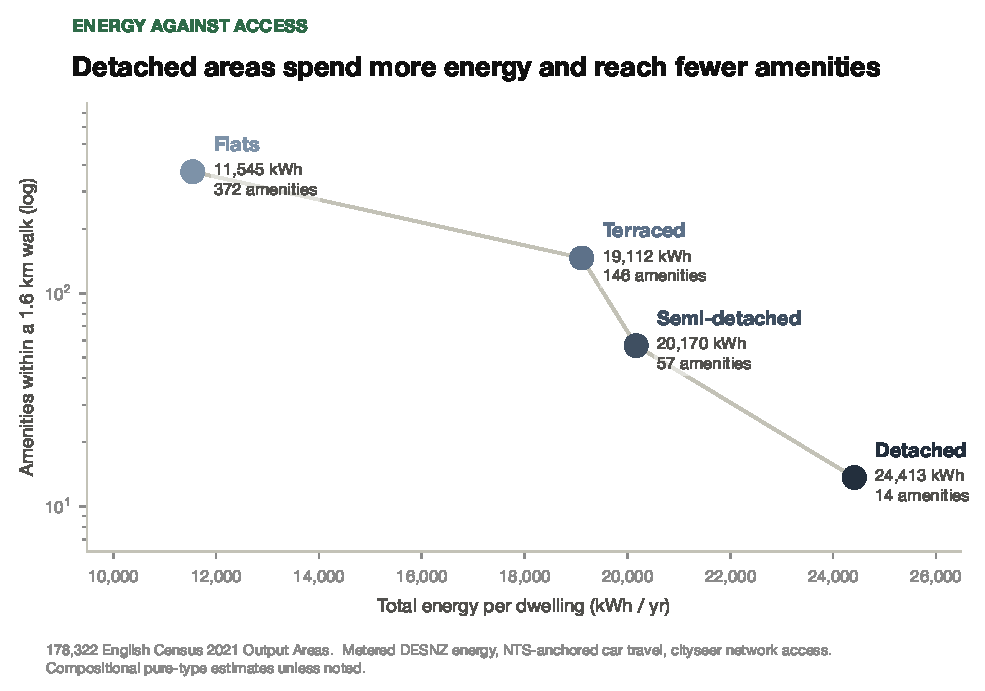
\includegraphics[width=\textwidth]{fig1_inversion}
  \caption{\textbf{Energy against access by dwelling type.} Regression estimates for neighbourhoods built wholly of each of the four principal dwelling types, with building age, deprivation, tenure, and climate held at their means (compositional pure-type predictions; Methods), across \nepisampleN{} English Census 2021 Output Areas: amenities of the benchmark basket (six everyday destination types, from general practitioners to grocery shops; Methods) within a 1.6\,km walk against total energy per dwelling. Energy rises and access falls from flats to detached houses: a detached neighbourhood uses about \nepitotalGapRound$\times$ the energy of a flat-type one and reaches 1/\nepiwalkAmenRound{} of the amenities.}
  \label{fig:inversion}
\end{figure}

\section*{Results}

The comparison covers the \nepisampleN{} of England's 178,605 Census 2021 Output Areas that hold more than ten residents and record positive metered consumption. In the great majority of cases, Output Areas represent a mixture of dwelling types, and the wholly-flat and wholly-detached extremes are rare, so a direct comparison between them is ambiguous. We therefore use a regression that reflects the composition of each area rather than a label for its dominant type. Each Output Area is described by the fractions of its homes that are flats, terraced, semi-detached, or detached, and the fitted model predicts what a neighbourhood built wholly of one type would consume once building age, deprivation, tenure, and local climate are held constant (Methods). The pure-type ratios therefore compare idealised extremes. Table~\ref{tab:axes} also reports the dominant-type median, the same contrast taken between the median flat-dominant and the median detached-dominant area as observed, so that the idealised ratios can be read against the actual data. Because adjacent Output Areas resemble one another, sharing weather, housing stock, and local policy, we compute the 95\% confidence intervals at the coarser scale of the \nepiclusters{} local-authority districts, so an interval narrows only where a ratio repeats across genuinely different places.

\subsection*{Energy}

Home energy, on which the policy instruments concentrate, shows a metered gap between forms of \nepiheatGap$\times$ (95\% CI \nepiheatGapCI). The headline figure includes three parts: larger dwellings, larger households, and a more exposed envelope. The gap falls to \nepiheatFamGap$\times$ (\nepiheatFamGapCI) when household size is held equal, and then to \nepiheatSizeGap$\times$ (\nepiheatSizeGapCI) when floor area is held equal on top of household size. We read what remains after both holds as largely the cost of the exposed envelope.

The larger share of the difference lies in travel, because residents of dispersed areas drive further. The National Travel Survey measures how far in each settlement class, and we disaggregate that mileage to Output Areas and convert it to energy at what the vehicle fleet consumes per mile (Methods); the car travel of a detached neighbourhood then comes to \nepitravelGap$\times$ (\nepitravelGapCI) that of a flat-type one. Unlike the home component, the contrast barely moves when household size is held equal, at \nepitravelFamGap$\times$. Together the components put total energy per dwelling at \nepitotalGap$\times$ (\nepitotalGapCI), or \nepifamNowGap$\times$ at equal household size (Table~\ref{tab:axes}). The same total can be read in reverse: the energy that houses one detached-type household would house about two flat-type households.

\begin{table}[!htbp]
  \caption{Access and energy by dwelling type. The four type columns give the median of the areas whose dominant (most common) dwelling type is the one named. The dominant-type median column is the ratio of the flat and detached medians, taken flat over detached for access and detached over flat for energy. The pure-type ratio is the compositional estimate for the idealised single-type extremes, with the confounds held (Methods). The final column repeats each energy ratio with household size held equal as a control; access belongs to the location, so it has no equal-household-size variant. Medians are not additive, so the energy total row, the per-area median of home plus travel, need not equal the sum of the home and travel rows.}
  \label{tab:axes}
  \centering
  {\footnotesize\setlength{\tabcolsep}{3pt}
    % Generated by the stats scripts via stats/ledger.py — do not edit.
% Regenerate by running the stats scripts (see paper/submission_checklist.md).
\begin{tabular}{lrrrrrr}
\toprule
 & Flat & Terraced & \shortstack[r]{Semi-\\detached} & Detached & \shortstack[r]{Dominant-\\type median} & \shortstack[r]{Pure-type\\ratio} \\
\midrule
\multicolumn{7}{l}{\textit{Access: opportunities within reach (median count)}} \\
Amenities, on foot & 184 & 101 & 57 & 19 & 9.7$\times$ & \nepiwalkAmen$\times$ \\
Amenities, own catchment & 2,234 & 1,935 & 2,358 & 2,313 & 1.0$\times$ & \nepicatchAmen$\times$ \\
Amenities, 25.6\,km drive & 18,029 & 8,522 & 7,460 & 3,906 & 4.6$\times$ & \nepidriveAmen$\times$ \\
Jobs, on foot & 6,928 & 3,790 & 2,101 & 598 & 11.6$\times$ & \nepiwalkJobs$\times$ \\
Jobs, 25.6\,km drive & 808,035 & 382,646 & 338,062 & 173,426 & 4.7$\times$ & \nepidriveJobs$\times$ \\
People, on foot & 17,841 & 11,861 & 8,208 & 2,766 & 6.4$\times$ & \nepiwalkPeople$\times$ \\
\botrule
\end{tabular}
\par\vspace{6pt}
  % Generated by the stats scripts via stats/ledger.py — do not edit.
% Regenerate by running the stats scripts (see paper/submission_checklist.md).
\begin{tabular}{lrrrrrrr}
\toprule
 & Flat & Terraced & \shortstack[r]{Semi-\\detached} & Detached & \shortstack[r]{Dominant-\\type median} & \shortstack[r]{Pure-type\\ratio} & \shortstack[r]{Equal\\household size} \\
\midrule
\multicolumn{8}{l}{\textit{Energy (kWh per dwelling per year)}} \\
Home energy & 10,194 & 12,995 & 13,876 & 15,020 & 1.47$\times$ & \nepiheatGap$\times$ & \nepiheatFamGap$\times$ \\
Car travel & 3,240 & 5,088 & 6,660 & 9,272 & 2.86$\times$ & \nepitravelGap$\times$ & \nepitravelFamGap$\times$ \\
Total & 13,674 & 18,265 & 20,564 & 23,832 & 1.74$\times$ & \nepitotalGap$\times$ & \nepifamNowGap$\times$ \\
\botrule
\end{tabular}
}
\end{table}

\subsection*{Access}

To measure access, we count the amenities, jobs, and people each neighbourhood can reach over the road network. The amenities are a benchmark basket of six everyday destination types, from general practitioners to grocery shops, counted identically for every neighbourhood in the country (Methods; Extended Data Table~1). A flat-type neighbourhood reaches \nepiwalkAmen$\times$ the amenities, \nepiwalkJobs$\times$ the jobs, and \nepiwalkPeople$\times$ the people of a detached-type one on foot, within 1,600\,m or a twenty-minute walk (95\% CIs in Fig.~\ref{fig:forest}; per-service counts in Extended Data Fig.~1). The amenities come out nearly equal, however, when counted at each type's own car catchment, set by how far its residents drive (\nepicatchAmen$\times$, 95\% CI \nepicatchAmenCI): residents of dispersed areas reach much the same range of amenities, and pay for it in energy. Nothing in the construction forces this convergence, because the distances come from the travel survey and the counts from the road network. When every area is instead given the same 25.6\,km drive, the flat-type area still reaches \nepidriveAmen$\times$ the amenities, \nepidriveJobs$\times$ the jobs, and \nepidrivePeople$\times$ the people (Table~\ref{tab:axes}, Fig.~\ref{fig:reach}). Figure~\ref{fig:map} maps both quantities across England (Extended Data Figs.~2 and~3).

\begin{figure}[!htbp]
  \centering
  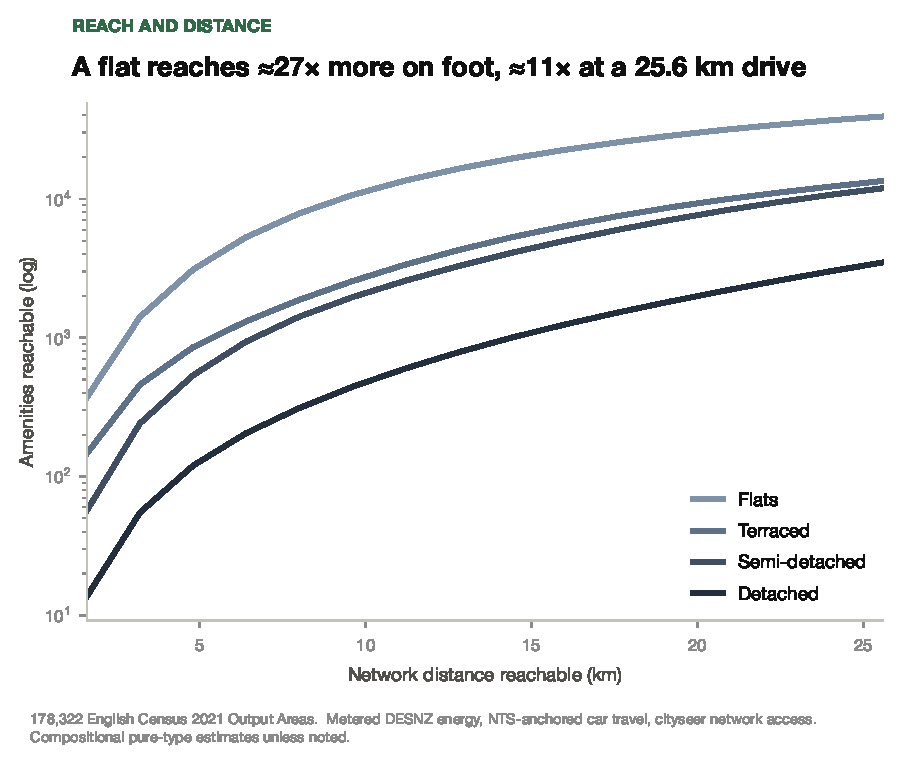
\includegraphics[width=0.85\textwidth]{fig6_access_curve}
  \caption{\textbf{Access against distance.} Amenities of the benchmark basket reachable against network distance, by dwelling type (compositional pure-type predictions): a flat-type neighbourhood reaches about \nepiwalkAmenRound$\times$ the amenities of a detached-type one on foot and \nepidriveAmenRound$\times$ at a 25.6\,km drive. The gap remains open at every distance shown.}
  \label{fig:reach}
\end{figure}

\begin{figure}[!htbp]
  \centering
  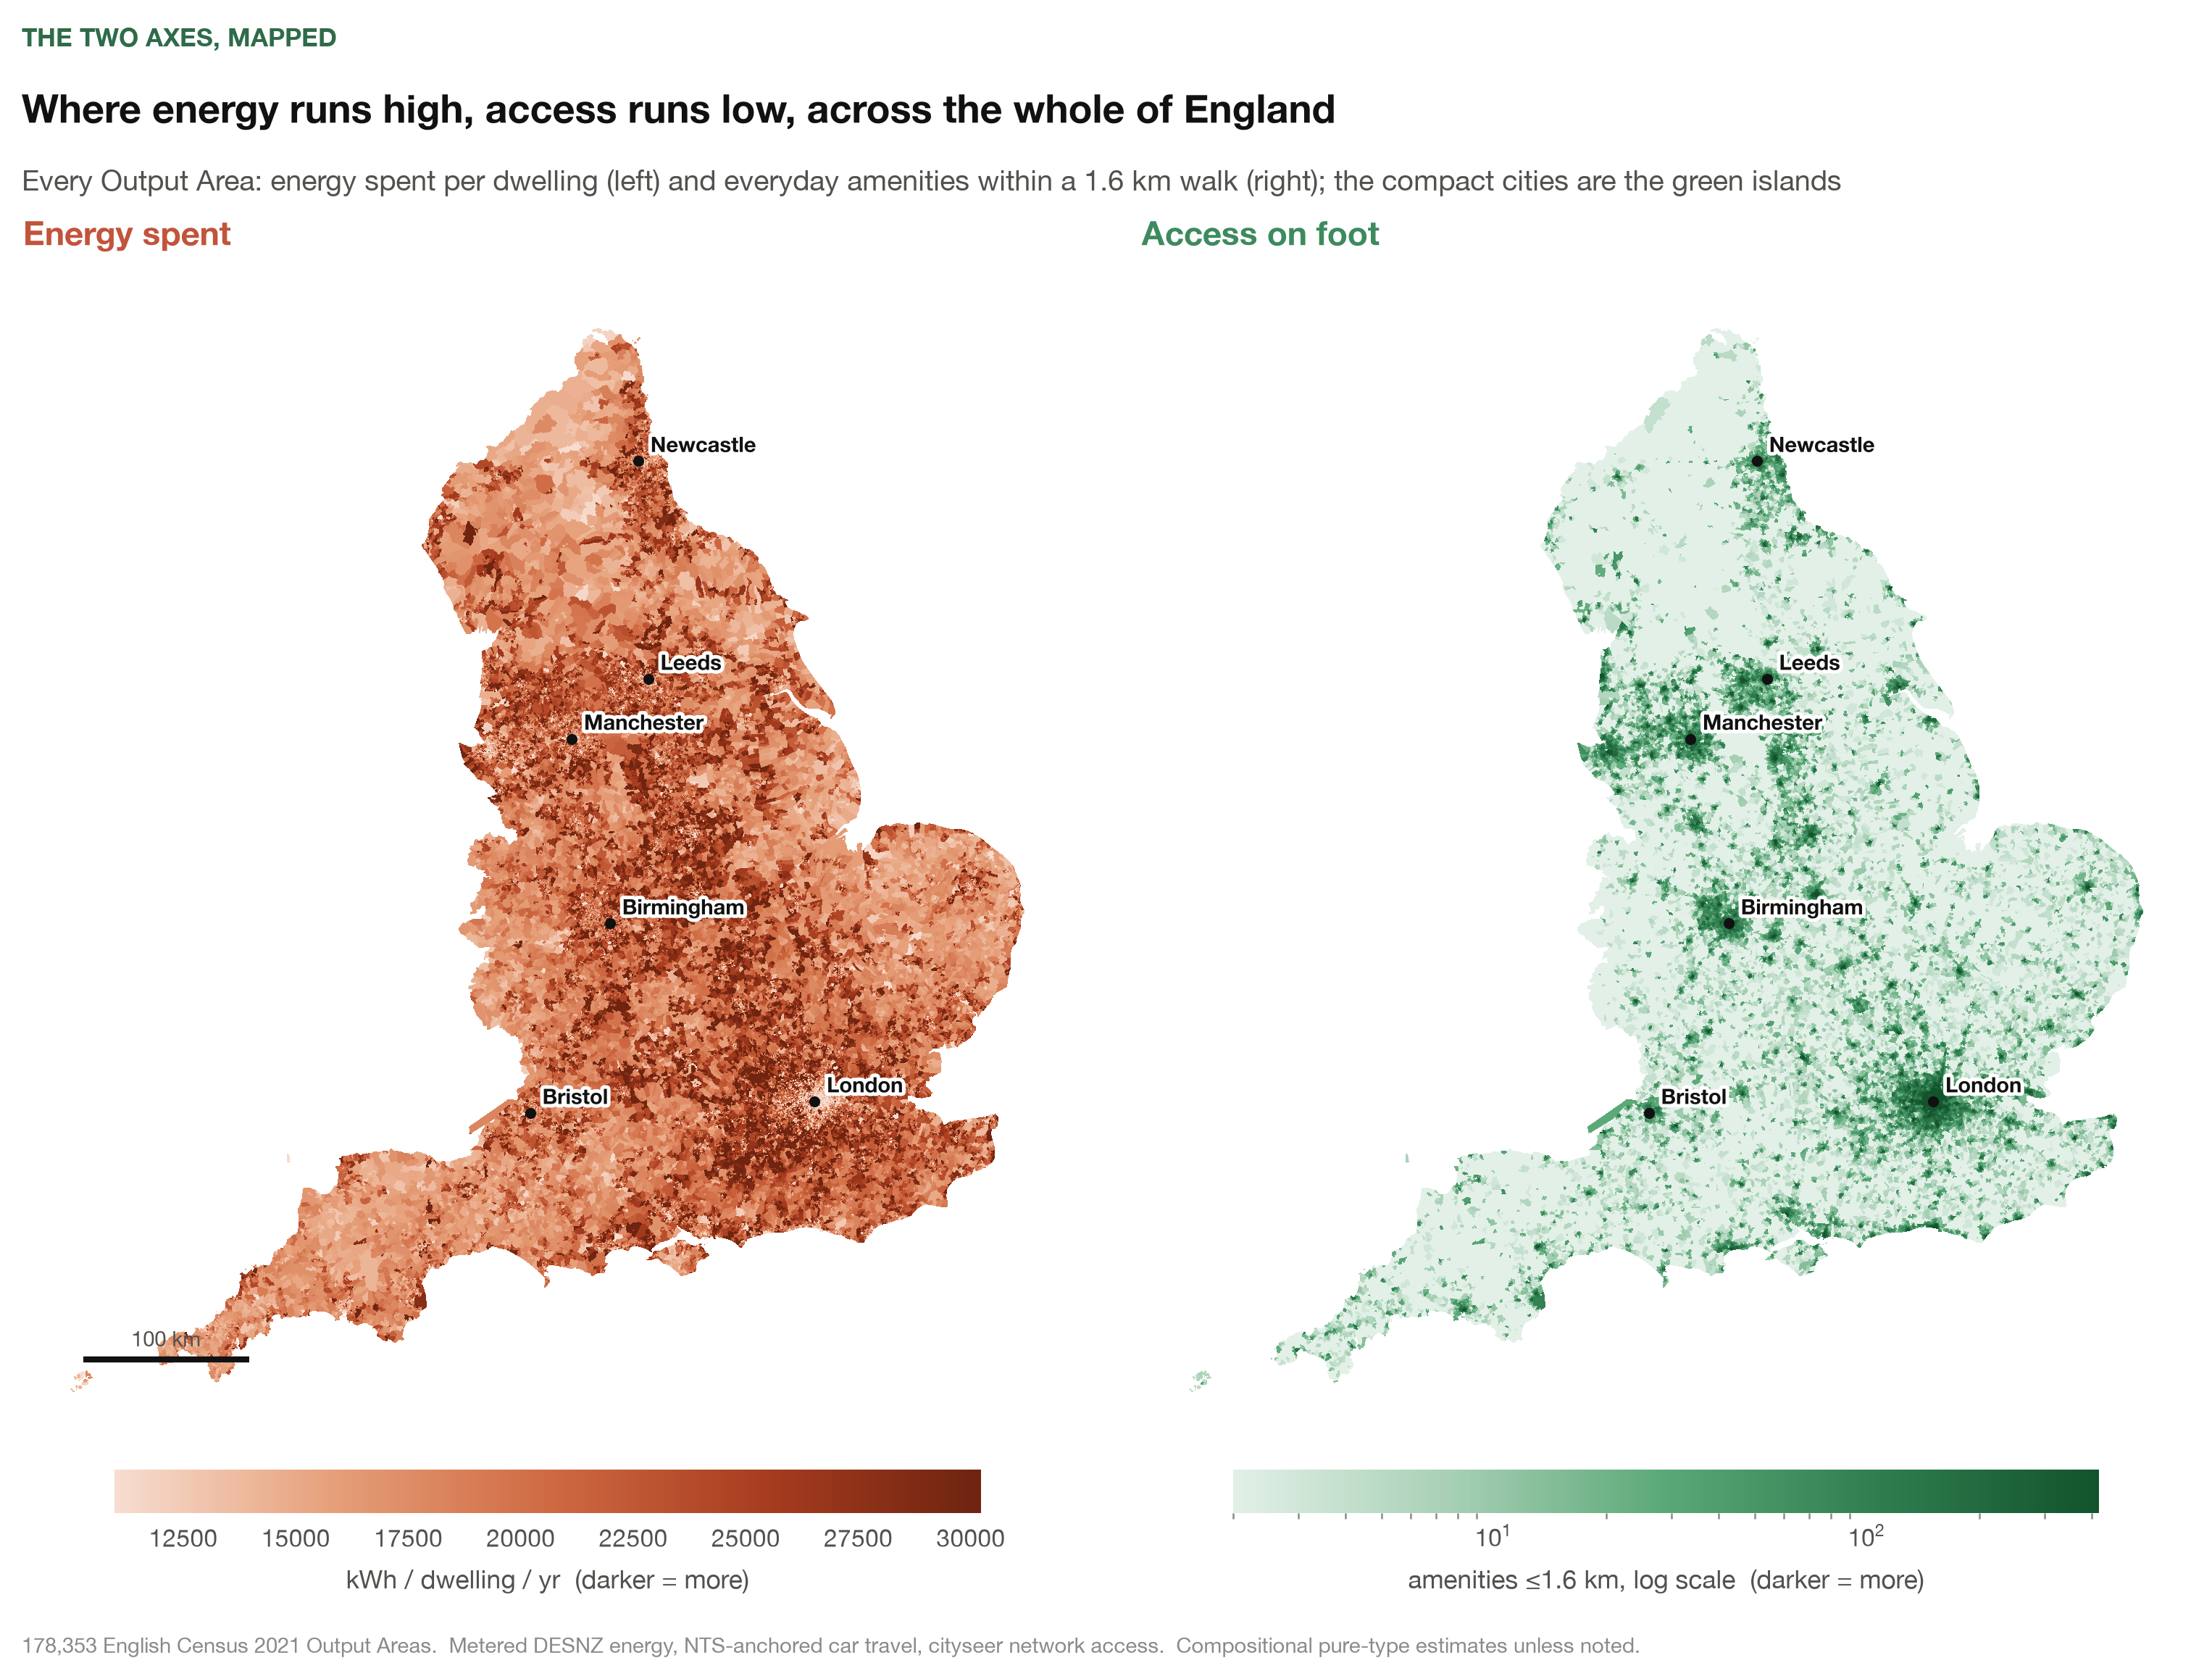
\includegraphics[width=\textwidth]{fig9_england.png}
  \caption{\textbf{Energy and access, mapped.} Each English Output Area is mapped by total energy (home plus car travel) per dwelling (left, continuous power-scaled colour ramp) and by amenities of the benchmark basket within a 1.6\,km walk (right, logarithmic colour scale). Dispersed high-energy form covers most of the land area, while walkable access is concentrated in the compact cities; the insets repeat Greater London on the same scales, aggregated to Lower-layer Super Output Areas for legibility.}
  \label{fig:map}
\end{figure}

\subsection*{The rate: access per kilowatt-hour}

Access per unit of energy is therefore the quantity that separates the forms. We divide the count of the benchmark basket within each area's own car catchment by its car-travel energy, the energy that buys access beyond walking distance. Within its catchment the flat-type area reaches slightly more amenities (\nepicatchAmen$\times$) while spending about a third of the energy, the \nepitravelGap$\times$ travel gap inverted. It therefore obtains $\nepicatchAmen \times \nepitravelGap \approx \nepirate\times$ (95\% CI \nepirateCI) the access per kilowatt-hour (Fig.~\ref{fig:rate}).

Driving enters both parts of the rate, the catchment within which the amenities are counted and the car-travel energy that divides them, so any error in the driving allocated to a given type would be amplified. We therefore recompute the rate with a denominator that deliberately de-emphasises driving: total energy, home plus travel, with the travel part priced at an all-electric fleet, so that driving makes up only a small share of it. The flat-type advantage remains, at \nepirateCirc$\times$ (\nepirateCircCI), which shows it to be a property of the neighbourhoods rather than of the rate's construction (Methods).

\begin{figure}[!htbp]
  \centering
  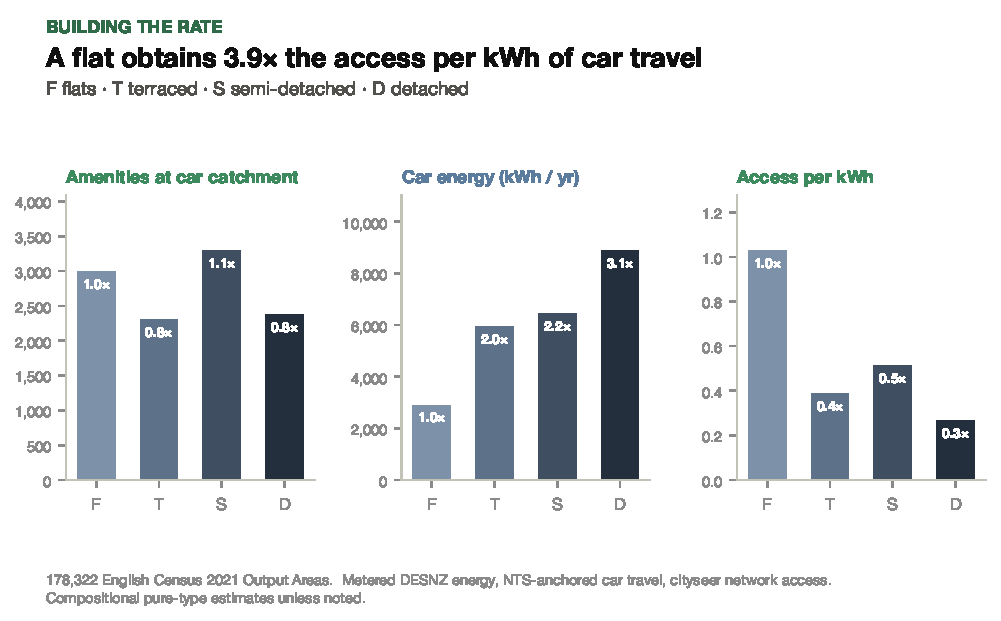
\includegraphics[width=0.85\textwidth]{fig7_rate}
  \caption{\textbf{The rate and its construction.} Amenities of the benchmark basket reachable at each area's own car catchment (left, nearly equal across types), the car-travel energy through which that reach is obtained (centre, \nepitravelGap$\times$ higher for detached), and the resulting access per kilowatt-hour (right): a flat-type area obtains about \nepirate$\times$ (95\% CI \nepirateCI) that of a detached-type one. The middle of the right panel falls out of type order because terraced and semi-detached areas differ more in car-travel energy than in the amenities their catchments reach. Compositional pure-type predictions; F, T, S, D denote flat, terraced, semi-detached, and detached.}
  \label{fig:rate}
\end{figure}

\subsection*{Decarbonisation scenarios and lock-in}

To test whether decarbonisation cancels the premium, and what lock-in remains, we recompute energy under each measure of the national strategy, alone and in combination (Methods; Fig.~\ref{fig:scenarios}). The measures leave the form of the neighbourhood unchanged, so access remains as measured. Consumption falls under every scenario, but the three measures act differently on the gap between forms. Insulation alone, deployed in full, closes more of the gap than any other single measure, moving it from \nepiscenarioBase$\times$ to \nepifabricGap$\times$; vehicle electrification closes nearly as much, taking the same starting gap to \nepievGap$\times$. Heat pumps alone cut home energy sharply but near-uniformly, so home energy shrinks as a share of the total, the wider travel gap comes to dominate, and the total gap widens marginally to \nepihpGap$\times$. The Climate Change Committee's Balanced Pathway for 2040, advised for the legislated carbon budgets, sets half of homes on heat pumps and three-quarters of cars electric \citep{ccc2025}, which brings the gap to \nepicccGap$\times$ (per-scenario confidence intervals in Extended Data Table~2).

The lock-in is what remains at full deployment of all three measures: the total gap falls from \nepiscenarioBase$\times$ to \nepifullGap$\times$ (\nepifullGapCI), so \nepifullSurvives\% of it survives, where the share is measured on the logarithmic scale of the ratio (Methods). Part of that gap exists because detached homes hold larger households, so we repeat the exercise with household size held equal, and full deployment then brings the gap down from \nepifamNowGap$\times$ to \nepifullFamGap$\times$ (\nepifullFamGapCI). The premium remains notable by the bar set in the introduction. Among the middle half of like areas, matched on composition, age, deprivation, tenure, and climate, the highest energy use is \nepiwithinSpread{} times the lowest even when all are fully treated. The surviving gap of \nepifullGap$\times$ is wider than that whole band, so the flat-type and detached-type bands do not meet (Extended Data Fig.~4). They would meet only if each band were widened from the middle half of its type's areas to the central \nepibandTouchShare\%. The band narrows to \nepiwithinSpreadFam{} when household sizes are held equal, in which case the gap still sits outside it (Methods).

\begin{figure}[!htbp]
  \centering
  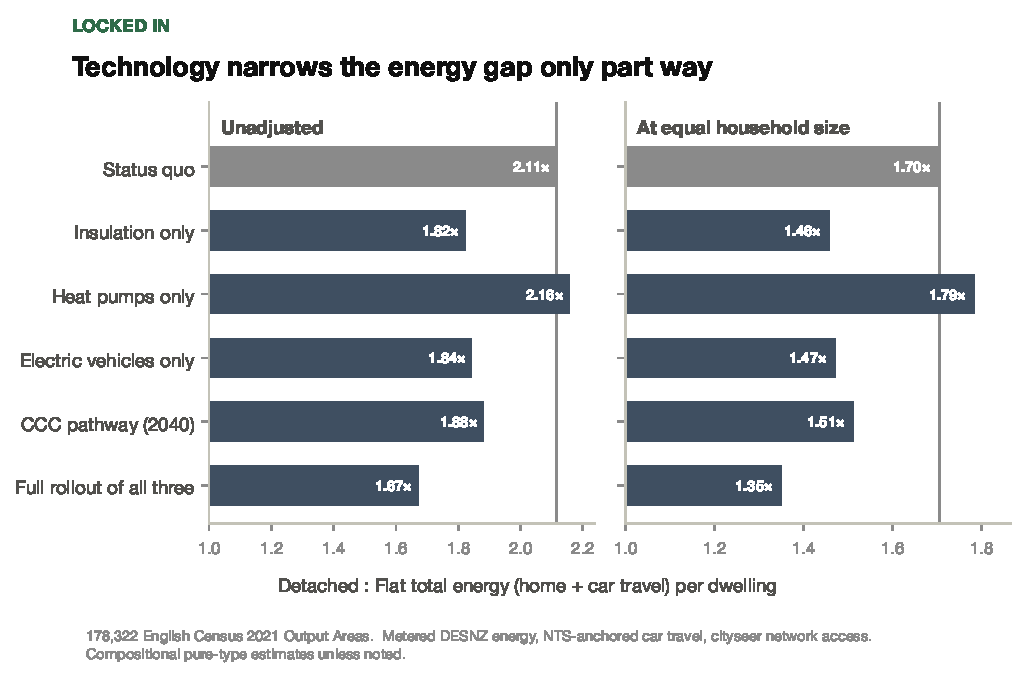
\includegraphics[width=0.85\textwidth]{fig8_scenarios}
  \caption{\textbf{The energy gap under each decarbonisation measure.} Bars show compositional detached:flat pure-type ratios of total energy, unadjusted (left) and at equal household size (right); the vertical line marks each panel's status-quo gap. Heat pumps alone widen the gap: they shrink home energy while leaving travel unchanged, so the larger travel gap shows through. The full-rollout bar, all three measures deployed in full, is the lock-in of \nepifullGap$\times$.}
  \label{fig:scenarios}
\end{figure}

\subsection*{Robustness}

Who lives where could produce the difference we attribute to form. If the households that choose detached houses are simply heavier energy users, in ways the controls---building age, income deprivation, tenure, and climate---do not record, the gap would describe them rather than their neighbourhoods. We check this in two ways. Adding occupational class, a strong marker of who lives where, leaves the gaps essentially unchanged. The measured controls themselves barely moved the gap, so an unrecorded difference would have to be as large as all of them together to remove it (coefficient-stability bound $\delta^{*} \approx \nepiosterDeltaTotal$ \citep{oster2019}). The home-energy gap alone would be more sensitive, but the claims are made on the total, in which travel is the larger part (Extended Data Table~3).

The travel gap could come from our own arithmetic, since driving is not observed at area level. It stays at or above \nepialphaZeroGap$\times$ (\nepialphaZeroGapCI), down from the headline \nepitravelGap$\times$, even when the allocation is flattened so that every area in a class receives the same per-person mileage (Extended Data Table~4). Adding public-transport energy, distributed the same way, leaves the total gap at \nepiptAssumedTotal$\times$ (\nepiptAssumedTotalCI), down from \nepitotalGap$\times$ (Extended Data Table~5).

Metering could bias the home-energy gap, because flat-type areas hold fewer domestic gas meters than households, and the consumption of a household without its own meter, as with communal heating, never enters the metered series. Restricting the sample to areas holding at least 0.9 gas meters per household raises the gap slightly, so the missing meters understate it (Extended Data Table~4).

The size of the areas compared could matter as well. Re-fitting the same model at the two coarser census geographies moves the total gap from \nepitotalGap$\times$ at Output Area scale to \nepimaupTotalLsoa$\times$ one level up and \nepimaupTotalMsoa$\times$ two levels up, so it narrows with aggregation but survives at every scale, although the home-energy contrast alone attenuates at the coarsest (Extended Data Table~6). Merging the districts into fifty contiguous spatial blocks widens the total-gap interval only slightly and leaves the estimate unchanged, so districts are a sufficient scale at which to compute the intervals (Methods). Figure~\ref{fig:forest} collects every headline ratio with its clustered confidence interval.

\begin{figure}[!htbp]
  \centering
  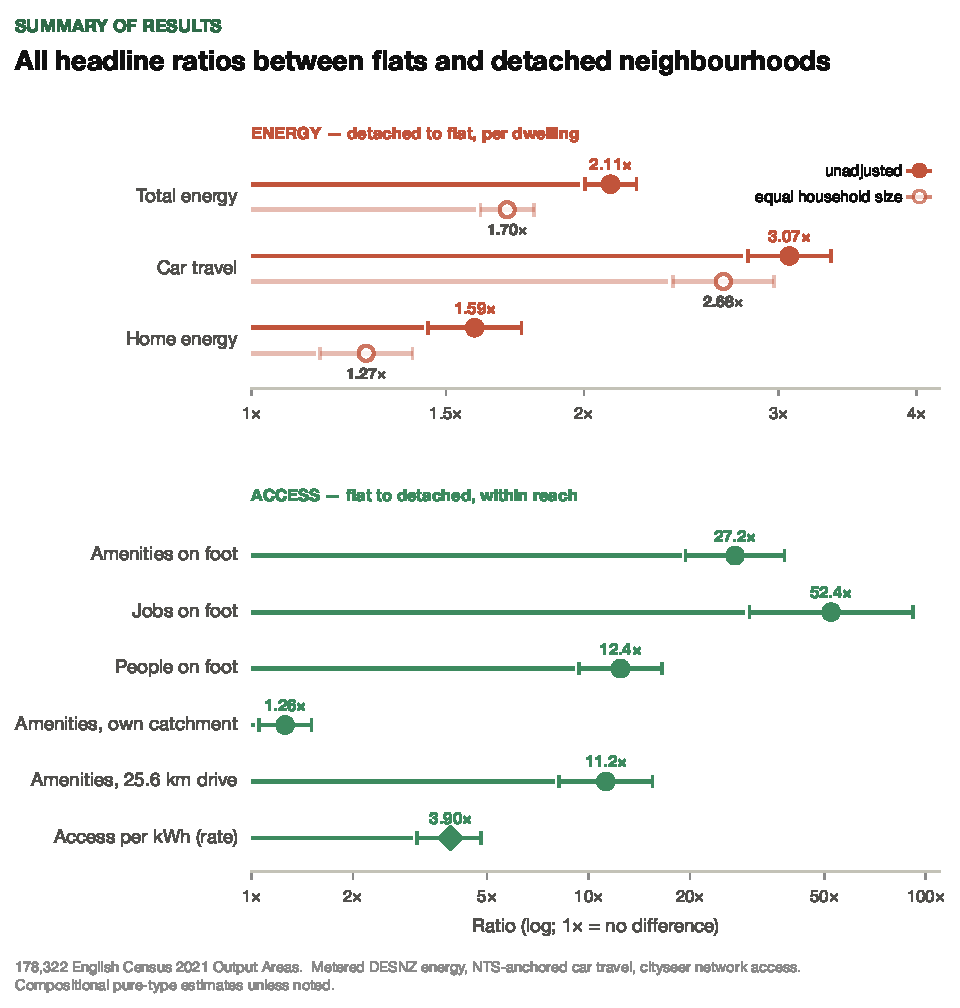
\includegraphics[width=0.85\textwidth]{fig11_forest}
  \caption{\textbf{All headline ratios with confidence intervals.} Compositional pure-type ratios with 95\% confidence intervals clustered on \nepiclusters{} local-authority districts: energy gaps (detached:flat, upper panel; filled markers unadjusted, open markers at equal household size) and access gaps (flat:detached, lower panel), each panel on its own logarithmic scale. The rate row (diamond) is the product of the catchment-amenity and car-travel rows; its interval comes from resampling whole districts rather than from propagating standard errors through the product (Methods).}
  \label{fig:forest}
\end{figure}

\section*{Discussion}

Measures applied to individual homes and vehicles do not cancel the energy premium of dispersed urban form. A detached-type neighbourhood uses \nepitotalGap$\times$ the energy of a flat-type one today, and full deployment of insulation, heat pumps, and electric vehicles leaves \nepifullGap$\times$. The on-foot access gap of \nepiwalkAmenRound$\times$ is unchanged in every scenario. The premium survives because the measures raise efficiency without changing the floor area to be heated or the distances to be driven, which are fixed by the building and the street layout and change only when places are rebuilt. This is lock-in in the strict sense \citep{unruh2000,seto2016}. A fully renewable grid would cut the emissions the premium causes without narrowing the premium.

The premium can be priced in plain units. After full deployment, a flat-type neighbourhood runs on about \nepifullFlatKwh{} kilowatt-hours per dwelling a year for homes and cars together, and a detached-type neighbourhood on about \nepifullDetKwh, a difference of roughly \nepifullPremiumKwh{} kilowatt-hours per dwelling. Multiplied across England's existing stock, that difference comes to about \nepistockPremiumTwh{} terawatt-hours a year, roughly a fifth of what the fully treated stock would use (Methods). Part of that total reflects household size rather than form, since detached homes house more people, and the premium from form alone is \nepistockFamPremiumTwh{} terawatt-hours a year. The existing stock turns over slowly, so that premium is committed for decades to come.

Current policy is geared to that existing stock and underplays form. For new development, where the lock-in can still be avoided, the omission has a price: every 100,000 dwellings built as detached-type rather than flat-type neighbourhoods add about \nepifullPremiumHundredK{} terawatt-hours a year for their lifetime. If the government's target of 1.5 million new homes over five years were built that way, the choice would add about 6 terawatt-hours a year, enough to run another million treated flat-type dwellings. % TODO: cite the 1.5M-homes housing target before submission.

Home energy can be checked against published measurement. National consumption statistics and metered regressions report detached gas consumption at about twice a flat's, with nothing held constant \citep{need2024,ehs2024,wyatt2013}; our \nepiheatGap$\times$ holds building age, deprivation, tenure, and climate, and the difference between the two figures is what those confounds explain. Counted per square metre the gap slightly reverses (\nepimSqGap$\times$), as the denominator literature reports \citep{norman2006}. Travel has no published counterpart at neighbourhood level, so its check comes from within the data. The counted amenities come out close together at each type's own catchment: about \nepicatchAmenFlat{} for flats, \nepicatchAmenTerr{} for terraced, \nepicatchAmenSemi{} for semi-detached, and \nepicatchAmenDet{} for detached areas (flat:detached \nepicatchAmen$\times$). This balance gives some assurance that the mileage disaggregation and the amenity counting are working as intended, since it reflects residents adjusting how far they drive to reach roughly equivalent amenities. As per the robustness checks, the gap narrows but does not close in the least favourable variants tested, with the mileage allocation flattened, public transport charged to residents, or the model re-fitted at the coarsest geography.

The instruments in current use act on home energy: certificates rate the dwelling's fabric, and subsidy pays to insulate it or to replace its boiler. Home energy is the smaller of the two gaps (Table~\ref{tab:axes}). The larger travel gap falls outside them, since it comes from where a neighbourhood is rather than from an asset a household owns and could upgrade. Current instruments also leave out the rate, which separates the forms most widely of all at \nepirate$\times$. Scoring neighbourhoods on their energy and their access would cover both, and would price proximity in kilowatt-hours, the unit in which retrofit and electrification are already appraised. We propose that the two quantities and the rate between them can be formalised as a neighbourhood energy performance index (NEPI).

Access ordinarily raises land prices and rents \citep{alonso1964}. Nationally, however, the distribution in England runs the other way, because deprivation is concentrated in compact form. The median area in the most income-deprived decile reaches about \nepiimdAccessRatio$\times$ the walkable amenities of the least deprived decile, while the least deprived decile uses \nepiimdEnergyRatio$\times$ the energy of the most deprived. Scoring access would therefore raise the value of the neighbourhoods where lower-income households already live, and they would pay for it in rents. Where housing markets are strongest, that revaluation has already occurred: the correlation between access and income deprivation is positive across England as a whole but near zero or negative in inner London, Manchester, and Bristol, where the least deprived areas hold the highest-access cores (Extended Data Fig.~5). Pricing proximity without expanding its supply would spread that pattern, pushing lower-income households out of the neighbourhoods the decarbonisation case favours. Planning for access therefore means expanding the supply of compact neighbourhoods as well as scoring the existing stock.

We identify the following limitations. Home energy is metered for every area, but car travel is measured by survey for each settlement class and allocated to the areas within it, so the travel component is constructed rather than observed at neighbourhood level. Travel energy counts car travel only, although charging public-transport energy to residents changes the gap little (Extended Data Table~5). The comparison is between places rather than households \citep{robinson1950,greenland2001}, so it cannot say what a household would use if it moved, and the definitive test, following movers in panel microdata, is out of scope. The insulation scenario treats each certificate's potential rating as fully achievable, which favours the measures, although taking it as a ratio to the current rating cancels the certificate's tendency to over-predict. Certificates cover about two-thirds of dwellings, and cover flats better than detached houses. Savings from efficiency are partly taken back in rebound, as households spend part of the saving on more warmth or travel, so dwelling-level gains need not scale to economy-wide reductions \citep{sorrell2007}. The analysis covers England only.

The energy productivity principle predicts that compact form obtains more use from an equivalent unit of energy, and the measured rate puts a figure on it. In the terms of the opening illustration, the dispersed neighbourhood is the desert, where an equivalent unit of energy streams through and yields a single use; the compact neighbourhood extracts \nepirate$\times$ the use from the same unit. These figures cover housing and access to land uses, and a fuller account of the complexity Jacobs described would likely place the advantage of compact form higher still. Decarbonisation strategy should therefore place greater emphasis on compact urban form and the access to amenities it affords.

\section*{Methods}

\subsection*{Unit of analysis}

The unit is the 2021 Census Output Area, the smallest published census geography, with about 125 households and 300 residents. Of England's 178,605 Output Areas, the \nepisampleN{} with more than ten residents and positive metered consumption are analysed. Wales is excluded because the English Index of Multiple Deprivation, used as a control, has no directly comparable Welsh equivalent. All inputs are open data, processed to the Output Area on the British National Grid (EPSG:27700): Census 2021 topic tables (population, household size, dwelling-type shares, tenure, occupational class, car ownership, commute distance, workplace jobs); DESNZ sub-national gas and electricity statistics; domestic Energy Performance Certificates (floor area, build year, current and potential intensity, aggregated as area medians); OS Open Roads; amenity registers (Food Standards Agency, Get Information about Schools, NHS Organisation Data Service, OS Open Greenspace); the Indices of Deprivation 2025; DVLA vehicle licensing; National Travel Survey table NTS9904; and HadUK-Grid 1991--2020 heating-degree-days.

\subsection*{Energy}

Energy is delivered energy in kilowatt-hours per dwelling per year, not primary energy or carbon. The home component is metered rather than modelled: postcode-level gas and electricity, each supplied as a meter count and a mean per meter, are aggregated to the Output Area by meter-weighted means, summed, and divided by census households. The gas series is corrected to a typical-weather year; the electricity series is not. Electricity is separated by meter profile class, the tariff categories that distinguish household from commercial meters. The domestic sector comprises the non-half-hourly standard and Economy 7 profiles, with meters on those profiles reallocated to the commercial sector above 100,000 kWh per year. Gas has no use-based flag; every meter consuming less than 73,200 kWh per year is classified as domestic, so small commercial premises remain in the domestic series. Such premises are concentrated in the compact areas that hold ground-floor commercial stock, and their consumption enters the numerator without adding to the household denominator, so the leakage inflates the measured energy of compact areas and can only shrink the reported gap.

The travel component is the total car-travel energy of a location's residents, not the commute alone (about one sixth of car mileage). It is anchored to the National Travel Survey, the Department for Transport's continuous survey of personal travel in England, in which each sampled household records a week of its trips in a travel diary and the results are weighted to represent the population. Driving is not observed at area level. Table NTS9904 gives measured car-driver miles per person for each of the six classes of the 2021 rural-urban classification of residence, from about 2,500 miles per person per year in the most urban class to 5,200 in the most rural. We share each class's mileage out among the neighbourhoods within it; this is the disaggregation. The sharing is constrained: the population-weighted mean of each class must reproduce the survey figure exactly, so the class totals are measured and only the distribution within a class is estimated. Mileage within a class is allocated by two markers of how much an area drives. The first is car ownership: allocated miles rise in proportion to an area's cars per person, so an area with twice the class's ownership receives twice the miles (an elasticity of one). The second is commute distance, taken as the mean of the census distance-band midpoints weighted by the number of commuters in each band. Its pull is weaker, at an elasticity of 0.30, so twice the commute distance draws about a quarter more miles. We set both elasticities rather than estimating them, and we sweep each one. The ownership elasticity is one because proportionality is the simplest defensible rule: an area with twice the cars per person is credited with twice the miles. Surveyed mileage in fact rises less than proportionally with additional cars, so proportionality pushes miles towards the high-ownership detached areas, and we sweep it down to zero, where only the measured between-class contrast remains (Extended Data Table~4). The commute elasticity is 0.30 because commuting accounts for about a sixth of car mileage and correlates with the rest, and we sweep it from 0.15 to 0.45. Because the survey counts miles per person and the unit here is the dwelling, allocated miles are multiplied by each area's census household size. Household size is therefore part of the per-dwelling travel contrast. Miles are converted to energy at the local fleet intensity, \nepitravelIce{} kWh per mile for internal combustion and \nepitravelEv{} for battery electric, blended by the DVLA battery-electric share and consistent with the Department for Transport's energy-consumption and appraisal tables. Metered domestic electricity already includes home electric-vehicle charging, so the travel figure double-counts that overlap; at the current battery-electric fleet share of 2--3\% the effect is negligible. Public-transport mileage from the same survey table is disaggregated in the same way, with the Census TS061 public-transport share of commuters as the within-class allocator, for the sensitivity reported in Extended Data Table~5; it does not enter the headline energy total.

\subsection*{Access}

Access is the count of opportunities reachable from an Output Area over the road network. The England network (OS Open Roads, about 3.6 million nodes) is built once into a routable graph (cityseer \citep{simons2023}), and counts are accumulated outwards from each Output Area's nearest node at 1,600\,m intervals up to 25,600\,m, with a count at an intermediate distance interpolated linearly between the two neighbouring rungs. Amenities are a benchmark basket of six everyday destination types, counted identically for every Output Area: general practitioners and pharmacies (NHS), schools (GIAS), places to eat and drink and grocery shops (FSA), and public parks and greenspace (Ordnance Survey); sources, record counts, and filters are given in Extended Data Table~1. Jobs are workplace jobs, counted at their workplace point and weighted by the number of jobs there. People are resident population, counted at each Output Area's centroid. Each is read at 1,600\,m, at the area's own car catchment, and at 25,600\,m.

\subsection*{The rate}

For each Output Area, the rate is the amenity count within the area's own car catchment divided by its car-travel energy. The catchment is the area's allocated annual car-driver distance per person divided by 370 trips per person per year, approximating the National Travel Survey car-driver trip rate (table NTS0303: 363 in 2023, about 380 before the pandemic). The resulting one-way distance is used as the network reach, bounded below at 1,600\,m and above at 25,600\,m. Recomputing the catchments at 300 and 440 trips per year moves the rate only from \nepitripMidRate$\times$ to \nepitripLowRate$\times$ and \nepitripHighRate$\times$, so the level of the constant has little effect. The flat-to-detached contrast of the rate is the product of two ratios already reported, the catchment amenities (flat:detached) and the car-travel energy (detached:flat), so it comes from Table~\ref{tab:axes} rather than from a separate model. Both of its ingredients depend on how far residents drive: the distance sets the catchment radius and, with the fleet intensity, the energy. One variant checks how much the rate owes to that shared ingredient. It replaces the denominator with total energy, home plus travel at electric fleet intensity, in which driving is only a small share, and gives \nepirateCirc$\times$ (\nepirateCircCI). A second variant places the two factors under the same controls. The access model holds the income domain alone (see the compositional model below), so the energy ratio is re-estimated on the same basis, giving \nepirateHarm$\times$ (\nepirateHarmCI).

\subsection*{The compositional model}

All contrasts derive from one compositional, no-intercept regression on each Output Area's dwelling-type shares (flat, terraced, semi-detached, detached, residual) as fractions summing to one. Without an intercept, each coefficient is the estimated outcome of a neighbourhood composed entirely of one type, and the ratio is $\exp(b_{\mathrm{detached}} - b_{\mathrm{flat}})$. The confounds enter at their observed values rather than as deviations from their means, and shift both pure-type predictions equally, so the ratio does not depend on the levels at which they are held. Regressions are household-weighted. The dominant-type median is reported alongside: the ratio of medians between areas whose dominant dwelling type is flat and those whose dominant type is detached.

Energy enters the model in logarithms per dwelling, so each fitted ratio compares geometric means, in which a few extreme areas cannot dominate the contrast. The headline gap is per dwelling and holds neither household size nor floor area. Each enters instead in a reported variant, with its strength estimated from the data rather than imposed: household size in the equal-household-size column of every table, and floor area in the size-held home-energy contrast. Dividing energy by people or by floor area would instead assume that energy rises one-for-one with each, and it does not. The household-size elasticity of home energy, estimated within the model, is \nepihhElast, and its elasticity to an area's median dwelling floor area, from a bivariate regression on floor area alone, is \nepifloorElast. Doubling either raises home energy by less than half again. Four confounds are held throughout: building age, deprivation (the overall Index of Multiple Deprivation and its income domain), tenure (social- and private-rented shares), and climate (heating-degree-days). Access counts are non-negative with frequent zeros, so they are fitted with a Poisson log link, the standard form for counts. Households enter as analytic weights, and the covariance is the cluster-robust sandwich, which stays valid when counts vary more than the Poisson form assumes. The access regression holds the income domain alone. Density is excluded because it is the mechanism under study, and the overall deprivation index because its barriers and living-environment sub-domains are themselves access measures.

Standard errors are clustered on the \nepiclusters{} local-authority districts, with $t(G-1)$ critical values; every reported ratio carries a 95\% interval on this basis. To check that districts are large enough to contain the spatial dependence, the total-gap interval was re-estimated with the districts merged into fifty contiguous spatial blocks (k-means on district centroids); the interval widens to \nepispatialBlockGapCI, from \nepitotalGapCI{} on districts, with the estimate unchanged. The rate carries a cluster-bootstrap interval with 999 replications, resampling whole districts; the per-scenario ratios carry their own clustered intervals (Extended Data Table~2). We give no interval for the percentage of the gap a scenario closes, because that percentage combines two fitted ratios and moves erratically when the districts are resampled.

\subsection*{Decarbonisation scenarios}

To test what decarbonisation leaves in place, we recompute energy under each measure and re-estimate the gap, holding access as measured. Insulation scales each area's metered gas by its fabric-improvement ratio, the area's median modelled potential intensity divided by its median modelled current intensity (median \nepifabricFactorMedian{} across areas). Ratios above one are set to one, so no area is made worse, and the ratio is floored at 0.1, so no area is credited with more than a tenfold improvement. Both terms come from the same model, so the certificate's tendency to over-predict divides out. Electricity is unchanged. Heat pumps replace each kilowatt-hour of gas with 0.32 kilowatt-hours of electricity. That factor is the boiler efficiency of 0.90 divided by a seasonal coefficient of performance of 2.8, the heat delivered per unit of electricity averaged over the year, and a sensitivity analysis varies the coefficient between 2.4 and 3.2 (Extended Data Table~2). Electrification prices car energy at the electric fleet intensity, with mileage unchanged. Both heat measures act on metered gas only, so electrically heated homes, more common among flats, keep their energy unimproved, which can only understate the surviving gap. Partial uptake blends transformed and untransformed energy linearly, and the Balanced Pathway scenario takes its 2040 stock shares from the Climate Change Committee, half of homes on a heat pump and three-quarters of cars electric \citep{ccc2025}.

\subsection*{Measuring what the scenarios leave}

Each measure multiplies energy by a factor, so the measures add on the logarithmic scale, where equality between the forms sits at zero. Shares of the gap closed or surviving are therefore measured in logarithms of the ratio. The alternative convention counts the share of the excess above equality that survives, $(r-1)/(r_{0}-1)$ for a surviving ratio $r$ and a starting ratio $r_{0}$, and gives \nepifullSurvivesExcess\% under the full rollout against the \nepifullSurvives\% reported on the logarithmic scale. Every scenario is fitted on one common complete-case sample (\nepiscenarioN{} areas with both a valid fabric ratio and a travel figure). Access is unchanged in every scenario.

The sufficiency bar compares the surviving gap with the band of variation among like neighbourhoods. We take the residuals of the same fit that produces the gap, in which composition and the confounds are already held, and report the band as the factor between the 25th and 75th percentiles of those residuals; outlying areas fall outside that middle half, so they cannot widen the band. The gap is also expressed in residual standard deviations (\nepifullGapSd{} per dwelling, \nepifullFamGapSd{} at equal household size). Outliers can only inflate that spread, so the expression understates the separation. The meeting point reported in the Results is the coverage of the central residual band whose width equals the logarithmic gap. The residuals carry the noise of allocating postcode meters and survey mileage to areas, so the band overstates the real variation between like places and the bar errs in favour of the measures. The absolute premium is the difference between the two pure-type predictions of the full-rollout fit, read at household-weighted mean confounds. The stock-wide figure re-prices every area at wholly flat composition, keeping its own confounds and its own residual, and sums the difference over households, with each area also keeping its own household size in the equal-household-size variant; it prices the standing cost of dispersed form, and implies no rebuilding.

\subsection*{Robustness and the estimand}

The quantity estimated is a property of places: the energy and access of a neighbourhood type with the observed confounds held. It therefore cannot say what any household would use if it moved, and the risk is self-sorting, in which the people who choose detached houses, rather than the houses themselves, could produce the energy difference. Sorting does not apply to access, which depends on location alone. We bound the sorting effect on the energy gaps with two checks. Adding occupational class, the share of residents in higher and lower managerial, administrative and professional occupations, leaves the gaps essentially unchanged. The second check estimates how strong an unrecorded difference in who lives where would have to be, relative to the measured controls, to remove the gap, and reports that multiple as $\delta^{*}$ \citep{oster2019}. The compositional model has no centred $R^2$, so the bound is computed on a continuous detached-share gradient in an intercept specification, using the coefficient-based approximation with $R_{\max} = \min(1.3\tilde{R}^{2}, 1)$, where $\tilde{R}^{2}$ is the $R^{2}$ of the regression that holds the confounds. The Results report $\delta^{*}$, and Extended Data Table~3 reports the $\delta = 1$ bias-adjusted gap. Meters are not households, and the mismatch runs with dwelling type, so the home-energy gap is re-estimated three ways: on areas holding at least 0.9 gas meters per household, on areas whose electricity-meter count lies between 0.5 and 1.5 times their household count, and with consumption winsorised at the 99.5th percentile (Extended Data Table~4). Output Area boundaries are one of several possible zonations, so the analysis is also re-run on the two coarser census geographies, carrying every variable up as a household-weighted mean and re-fitting the identical model alongside the dominant-type median ratio at each scale (Extended Data Table~6).

\subsection*{Data availability}

All inputs are open data: Census 2021, DESNZ sub-national energy consumption statistics, domestic Energy Performance Certificates, NTS9904, DVLA vehicle licensing, the Indices of Deprivation 2025, HadUK-Grid, OS Open Roads, Open Greenspace, Open UPRN and Code-Point Open, the FSA food-hygiene register, GIAS, and the NHS Organisation Data Service. The built per-Output-Area artefacts will be deposited with a DOI on acceptance. % TODO: mint the deposit DOI before submission.

\subsection*{Code availability}

The acquisition pipeline, analysis scripts, and figure code are available at \url{https://github.com/UCL/urban-energy}. Analyses use Python 3.13 with cityseer, statsmodels, geopandas, pandas, and NumPy; the fully pinned environment is recorded in the repository lock file. % TODO: archive a tagged release with a DOI before submission.

\section*{Declarations}

\bmhead{Acknowledgements} % TODO
\bmhead{Author contributions} % TODO: CRediT statement once the author list is final.
\bmhead{Competing interests} The authors declare no competing interests.

\bibliography{../references}

\end{document}
